\chapter{Support Material for the Combined $VH(H\rightarrow b\bar{b}/c\bar{c})$ Analysis}
\textit{This Appendix lists some additional results in support of Chapter \ref{chap-VH}.}

\section{Triggers}\label{appsec-trigger}
This section gives further details on the triggers used in the combined analysis presented in Chapter \ref{chap-VH}.

\begin{table}[!htpb]
    \begin{center}
      \scriptsize
      \resizebox{\textwidth}{!}{
        \begin{tabular}{c|c|c|c|p{7.2cm}} \hline \hline
           \textbf{ Type } & \textbf{ Trigger Name }        &     \textbf{Period}     &  \textbf{Threshold}     &     \textbf{Description}               
          \\ \hline \hline
          \multirow{5}{*}{$\etm$}  
          & HLT\_xe70\_L1XE50         &      2015               &      70 GeV                    &    
          \multirow{5}{*}{\parbox{6.6cm}{Seeded using the level L1\_XE50 (L1\_XE55) LAr and Tile calorimeter triggers, 
                          calibrated at the EM scale, with a threshold of 50(55) GeV.}} \\
          & HLT\_xe90\_mht\_L1XE50         &      2016 (A-D3)               &      90 GeV                    &     \\
          & HLT\_xe110\_mht\_L1XE50        &      2016 ($\geq$ D4)              &      110 GeV                   &     \\
          & HLT\_xe110\_pufit\_L1XE55        &      2017               &      110 GeV                   &    \\
          & HLT\_xe110\_pufit\_xe70\_L1XE50        &      2018               &      110 GeV                   &    \\
          \hline \hline
          \multirow{7}{*}{Electron}  
          & HLT\_e24\_lhmedium\_L1EM20VH  &  2015  &   24 GeV    &    Seeded using L1 EM20VH level 1 trigger calibrated at the EM scale with a threshold of 20 GeV, require likelihood medium ID.\\
          & HLT\_e60\_lhmedium            &  2015  &   60 GeV    &    Require likelihood medium ID.\\
          & HLT\_e120\_lhloose            &  2015  &  120 GeV    &    Require likelihood loose ID.\\
          & HLT\_e26\_lhtight\_nod0\_ivarloose  &      2016 -- 2018         &         26 GeV     &    Tight likelihood ID required, alignment-robust likelihood tune with no d0 information used, and variable loose isolation required\\
          & HLT\_e60\_lhmedium(\_nod0)           &      2016 -- 2018        &         60 GeV     &    Medium ID likelihood required\\
          & HLT\_e140\_lhloose(\_nod0)           &      2016 -- 2018        &         140 GeV    &    Loose ID likelihood required\\
          & HLT\_e300\_etcut                     &      2018                &         300 GeV    &    No ID requirements. \\
          \hline \hline
          \multirow{3}{*}{Muon}  
          & HLT\_mu20\_iloose\_L1MU15      &      2015           &  20 GeV &   Seeded using L1MU15 level 1 trigger with a threshold of 15 GeV, and requiring loose isolation requirements.\\
          & HLT\_mu50\                     &      2015 -- 2018   &  50 GeV &   No isolation requirements. \\
          & HLT\_mu26\_ivarmedium          &      2016 -- 2018   &  26 GeV &   Variable cone medium isolation requirements \\
          \hline \hline
        \end{tabular}
      }
      \caption{Triggers used during the 2015-2018 data collection period, from the internal documentation.
               For the HLT that L1 trigger is not mentioned, the default L1 trigger is used. 
               The default L1 trigger is EM22VHI or EM24VHI for single electron, 
               MU20 or MU21 for single muon, depends on the data taken period
               \cite{TwikiTriggerNamingRun2}. }
      \label{tab:trigs2015_to_2018}
    \end{center}
  \end{table}

\section{Analysis Categorisation}\label{ap-vhCat}
This section offers more details in the categorisation of the $VH(H\rightarrow b\bar{b}/c\bar{c})$ Combined Analysis. The tagging requirements for an event to be in the \glsfirst{sr} are:
\begin{itemize}
\item For $VH(H\rightarrow b\bar{b})$, strictly two jets must be $b$-tagged and no tight $c$-tagged jets are allowed. 
\item For $VH(H\rightarrow c\bar{c})$, no $b$-tagged jets are allowed and at least one jet must be tight $c$-tagged. This defines three possible signal regions, where a second jet is either tight $c$-tagged ($TT$), loose $c$-tagged ($LT$), or not tagged ($TN$). 
\end{itemize}
Two control regions are defined by modifying the conditions on the tags of the jets in the event: 
\begin{itemize}
\item A combined $VH(H\rightarrow b\bar{b})$ and $VH(H\rightarrow c\bar{c})$ top control region (topCR) is obtained by requiring at least 1 $b$-tagged jet and 1 $c$-tagged jet. The definition of this control region is the core subject of this work and will be further addressed later in this report. 
\item For $VH(H\rightarrow c\bar{c})$ only, an additional control region is defined by requiring a loose $c$-tagged and a non $b$- nor $c$-tagged jets in the event to constrain the significant $V$+light-jet background. 
\end{itemize}

\subsection{The $\Delta R$ Cut Between Higgs Candidate Jets}\label{ap-sec-vh-deltaR}
The angular separation between the two candidate jets $\Delta R(j_1, j_2)$, as defined in Equation \ref{eq-deltaR}, can be used to define a control region enriched in $V$+jets and $t\bar{t}$ backgrounds since these two processes give candidate jets with a flat angular spectrum while the signal peaks at low values of $\Delta R$. A \textit{high $\Delta R$} control region (High $\Delta R$ CR) is defined using parametrised cuts on $\Delta R$ between the Higgs candidate jets as a function of $p_T^V$. An additional \textit{low $\Delta R$} control region (Low $\Delta R$ CR) for the 1L channel in $VH (H\rightarrow b\bar{b})$ resolved is also introduced (it is merged with the signal region for the $VH (H\rightarrow c\bar{c})$). The philosophy behind the parametrisation of this function is to adapt the cut on the expected angular separation between the two Higgs candidate jets as a function of how boosted they are, as described by the $p_T^V$ variable. For signal events, we expect the $H$ and $V$ to be approximately back-to-back hence $p_T^V$ is a good proxy for $p_T^H$ while benefiting from better experimental resolution, as it is reconstructed from leptons $p_T$ and/or $E_T$, depending on the channel. From physical principals, boosted candidate jets are indeed expected to have a lower angular separation. From the point of view of $VH (H\rightarrow c\bar{c})$, this modified cut represents a significant modification to the standalone analysis that relied on a simple fixed $\Delta R_{c\bar{c}}$ cut. The new cuts are defined by fitting a template function $ c_1 \times e^{c_2 + c_3 \times p_T^V}$ so that:   
\begin{itemize}
\item 95\% (85\%) of the $VH(H\rightarrow c\bar{c})$ signal is below the top limit for the 2-jet (3-jet) signal region,
\item 90\% of the diboson process is above the bottom limit in both signal regions.
\end{itemize}

The results of these fits for the 1L channel are displayed in Figure \ref{fig:drccptvCutsVHcc}, showing the signal yield in a 2-dimensional histogram ($p_T^V$ vs $\Delta R_{c\bar{c}}$) for different tags applied. The cut used in $VH(H\rightarrow b\bar{b})$, in yellow, shows a good agreement with the one derived on the $TT$-tagged (tight-tight) events in cyan and the $LT$-tagged (loose-tight) in green. The $VH(H\rightarrow b\bar{b})$ cuts is chosen so that the kinematic selection of the two analyses is harmonised. In $VH (H\rightarrow c\bar{c})$, the low $\Delta R$ CR does not improve the statistical significance hence this region is merged with the signal region. In $VH(H\rightarrow b\bar{b})$, these CRs are used to extract the normalisation of the backgrounds while in $VH (H\rightarrow c\bar{c})$ the shape of the $m_{c\bar{c}}$ spectrum is also used.  \\

\begin{figure}[h!]
%\hspace{-2.0cm}
\center
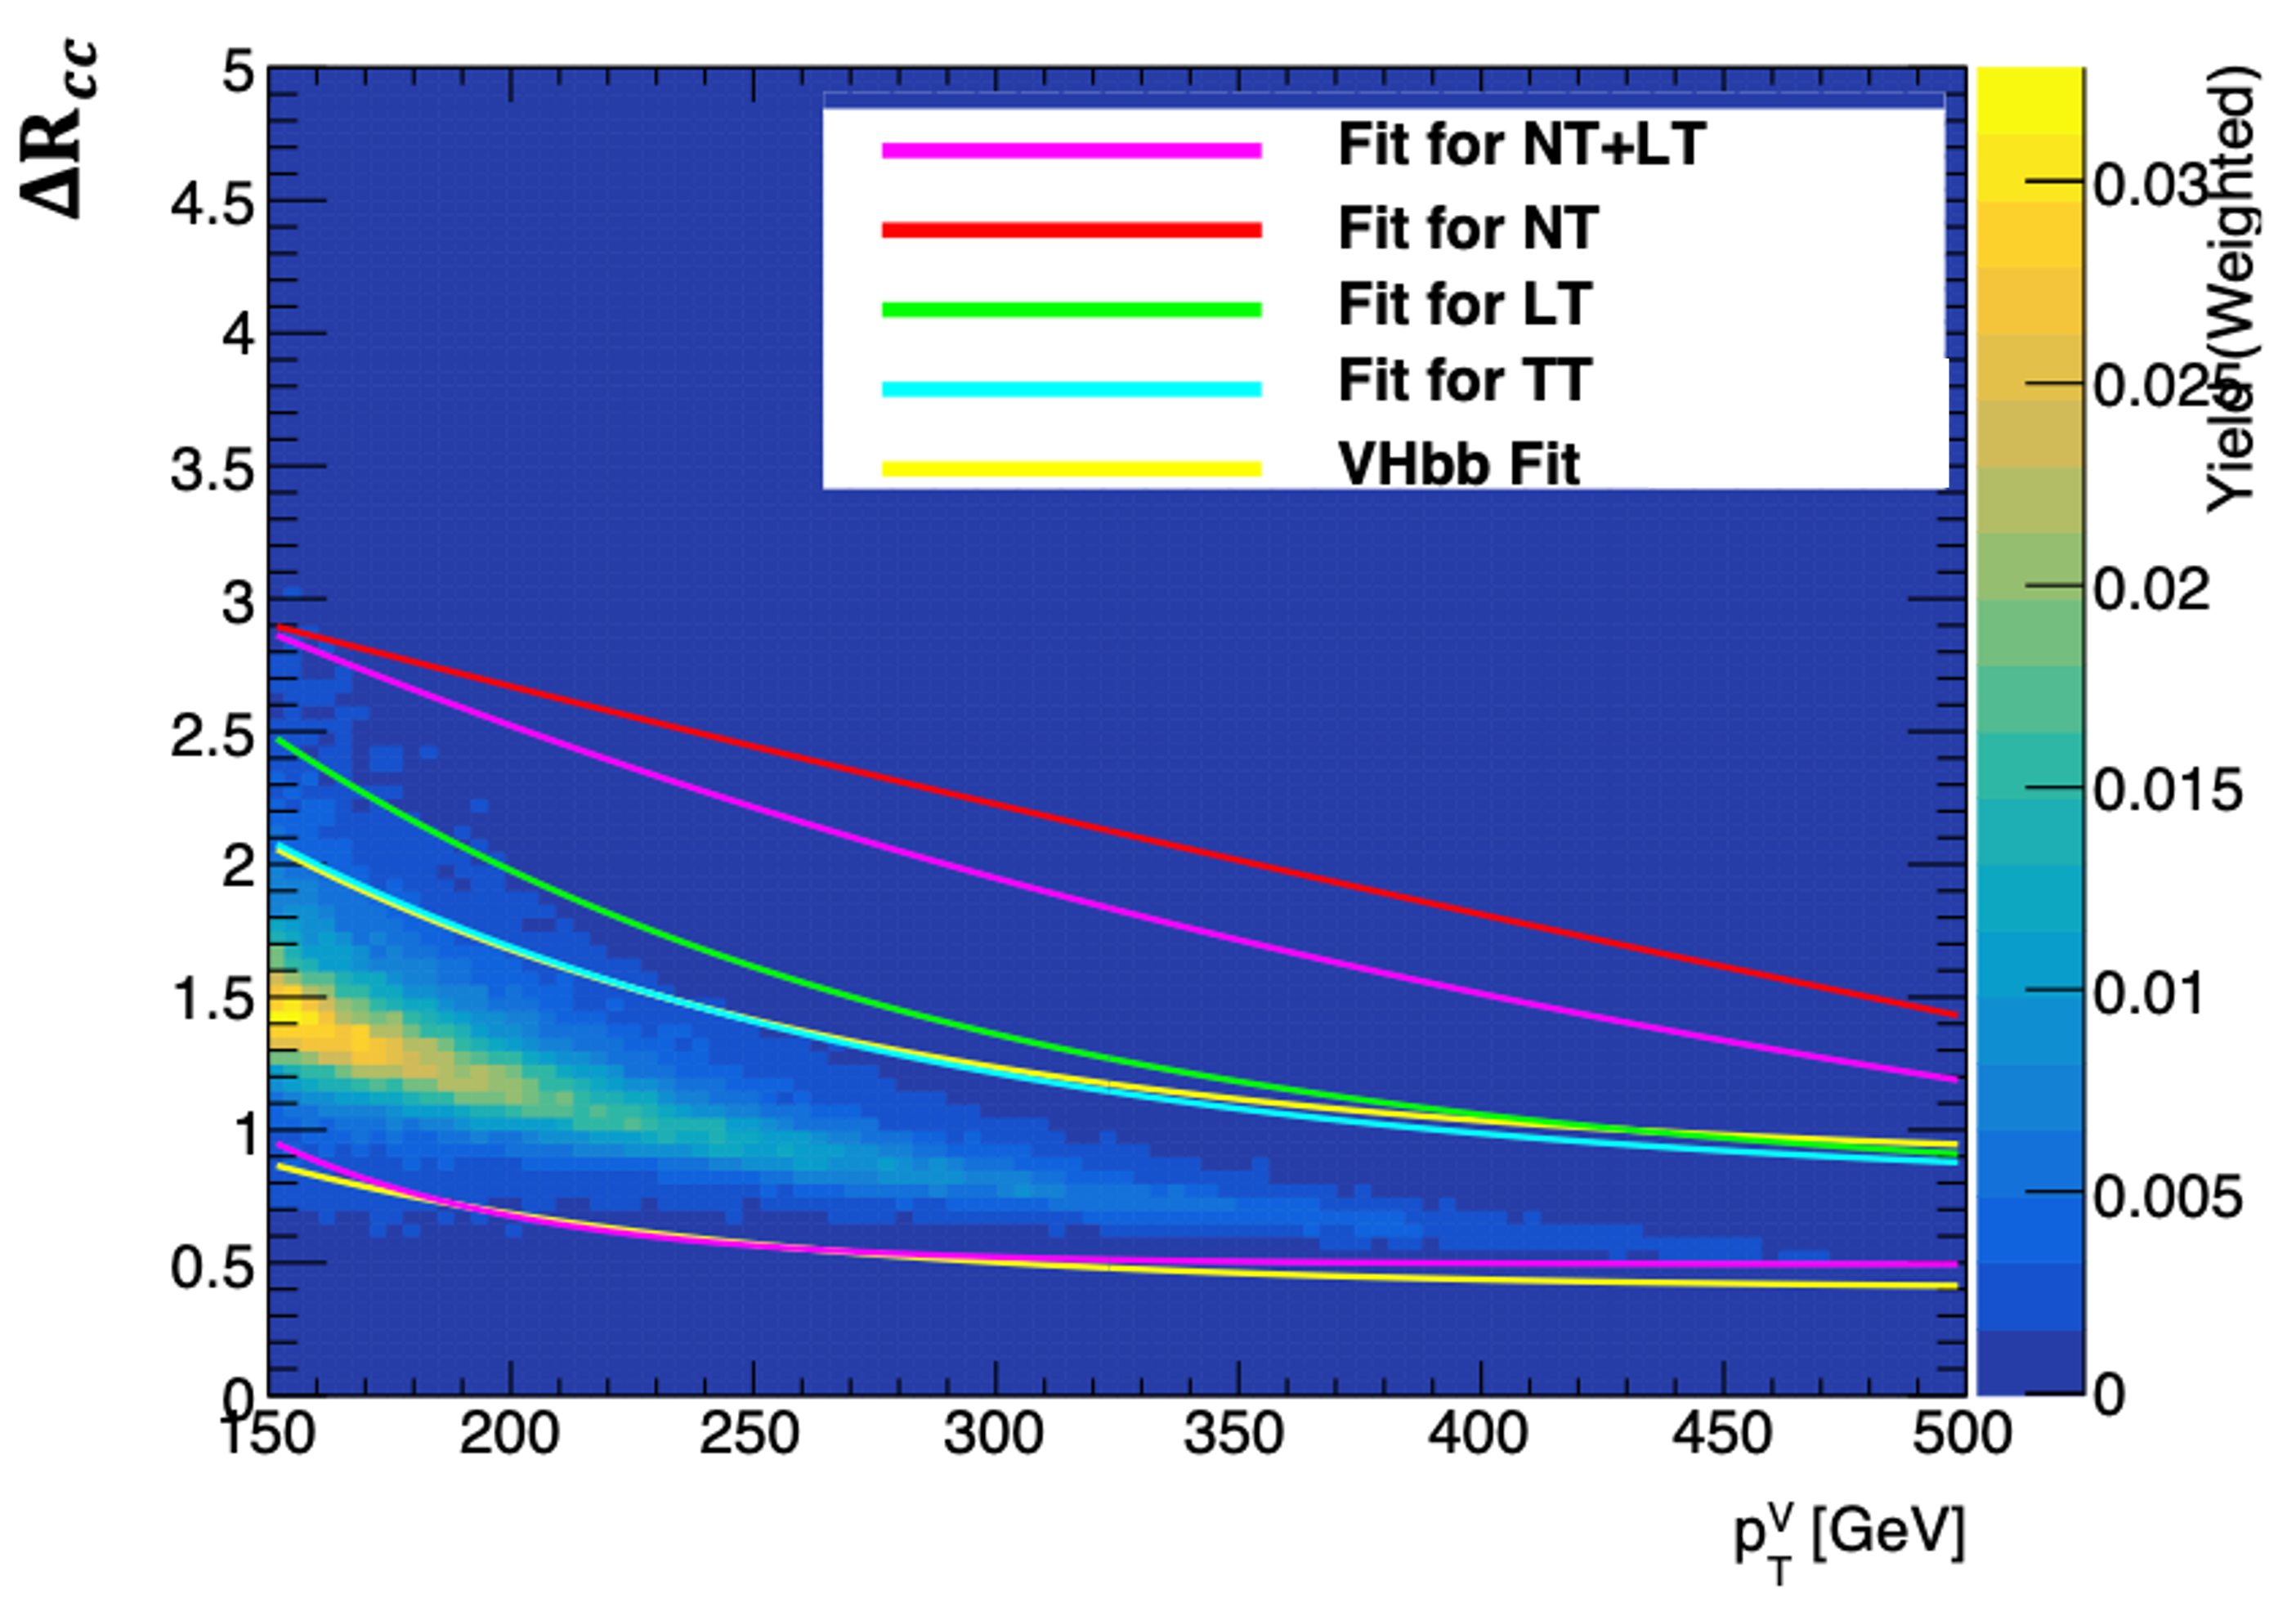
\includegraphics[width=0.48\textwidth]{Images/VH/dRccpTV/sr1.png}
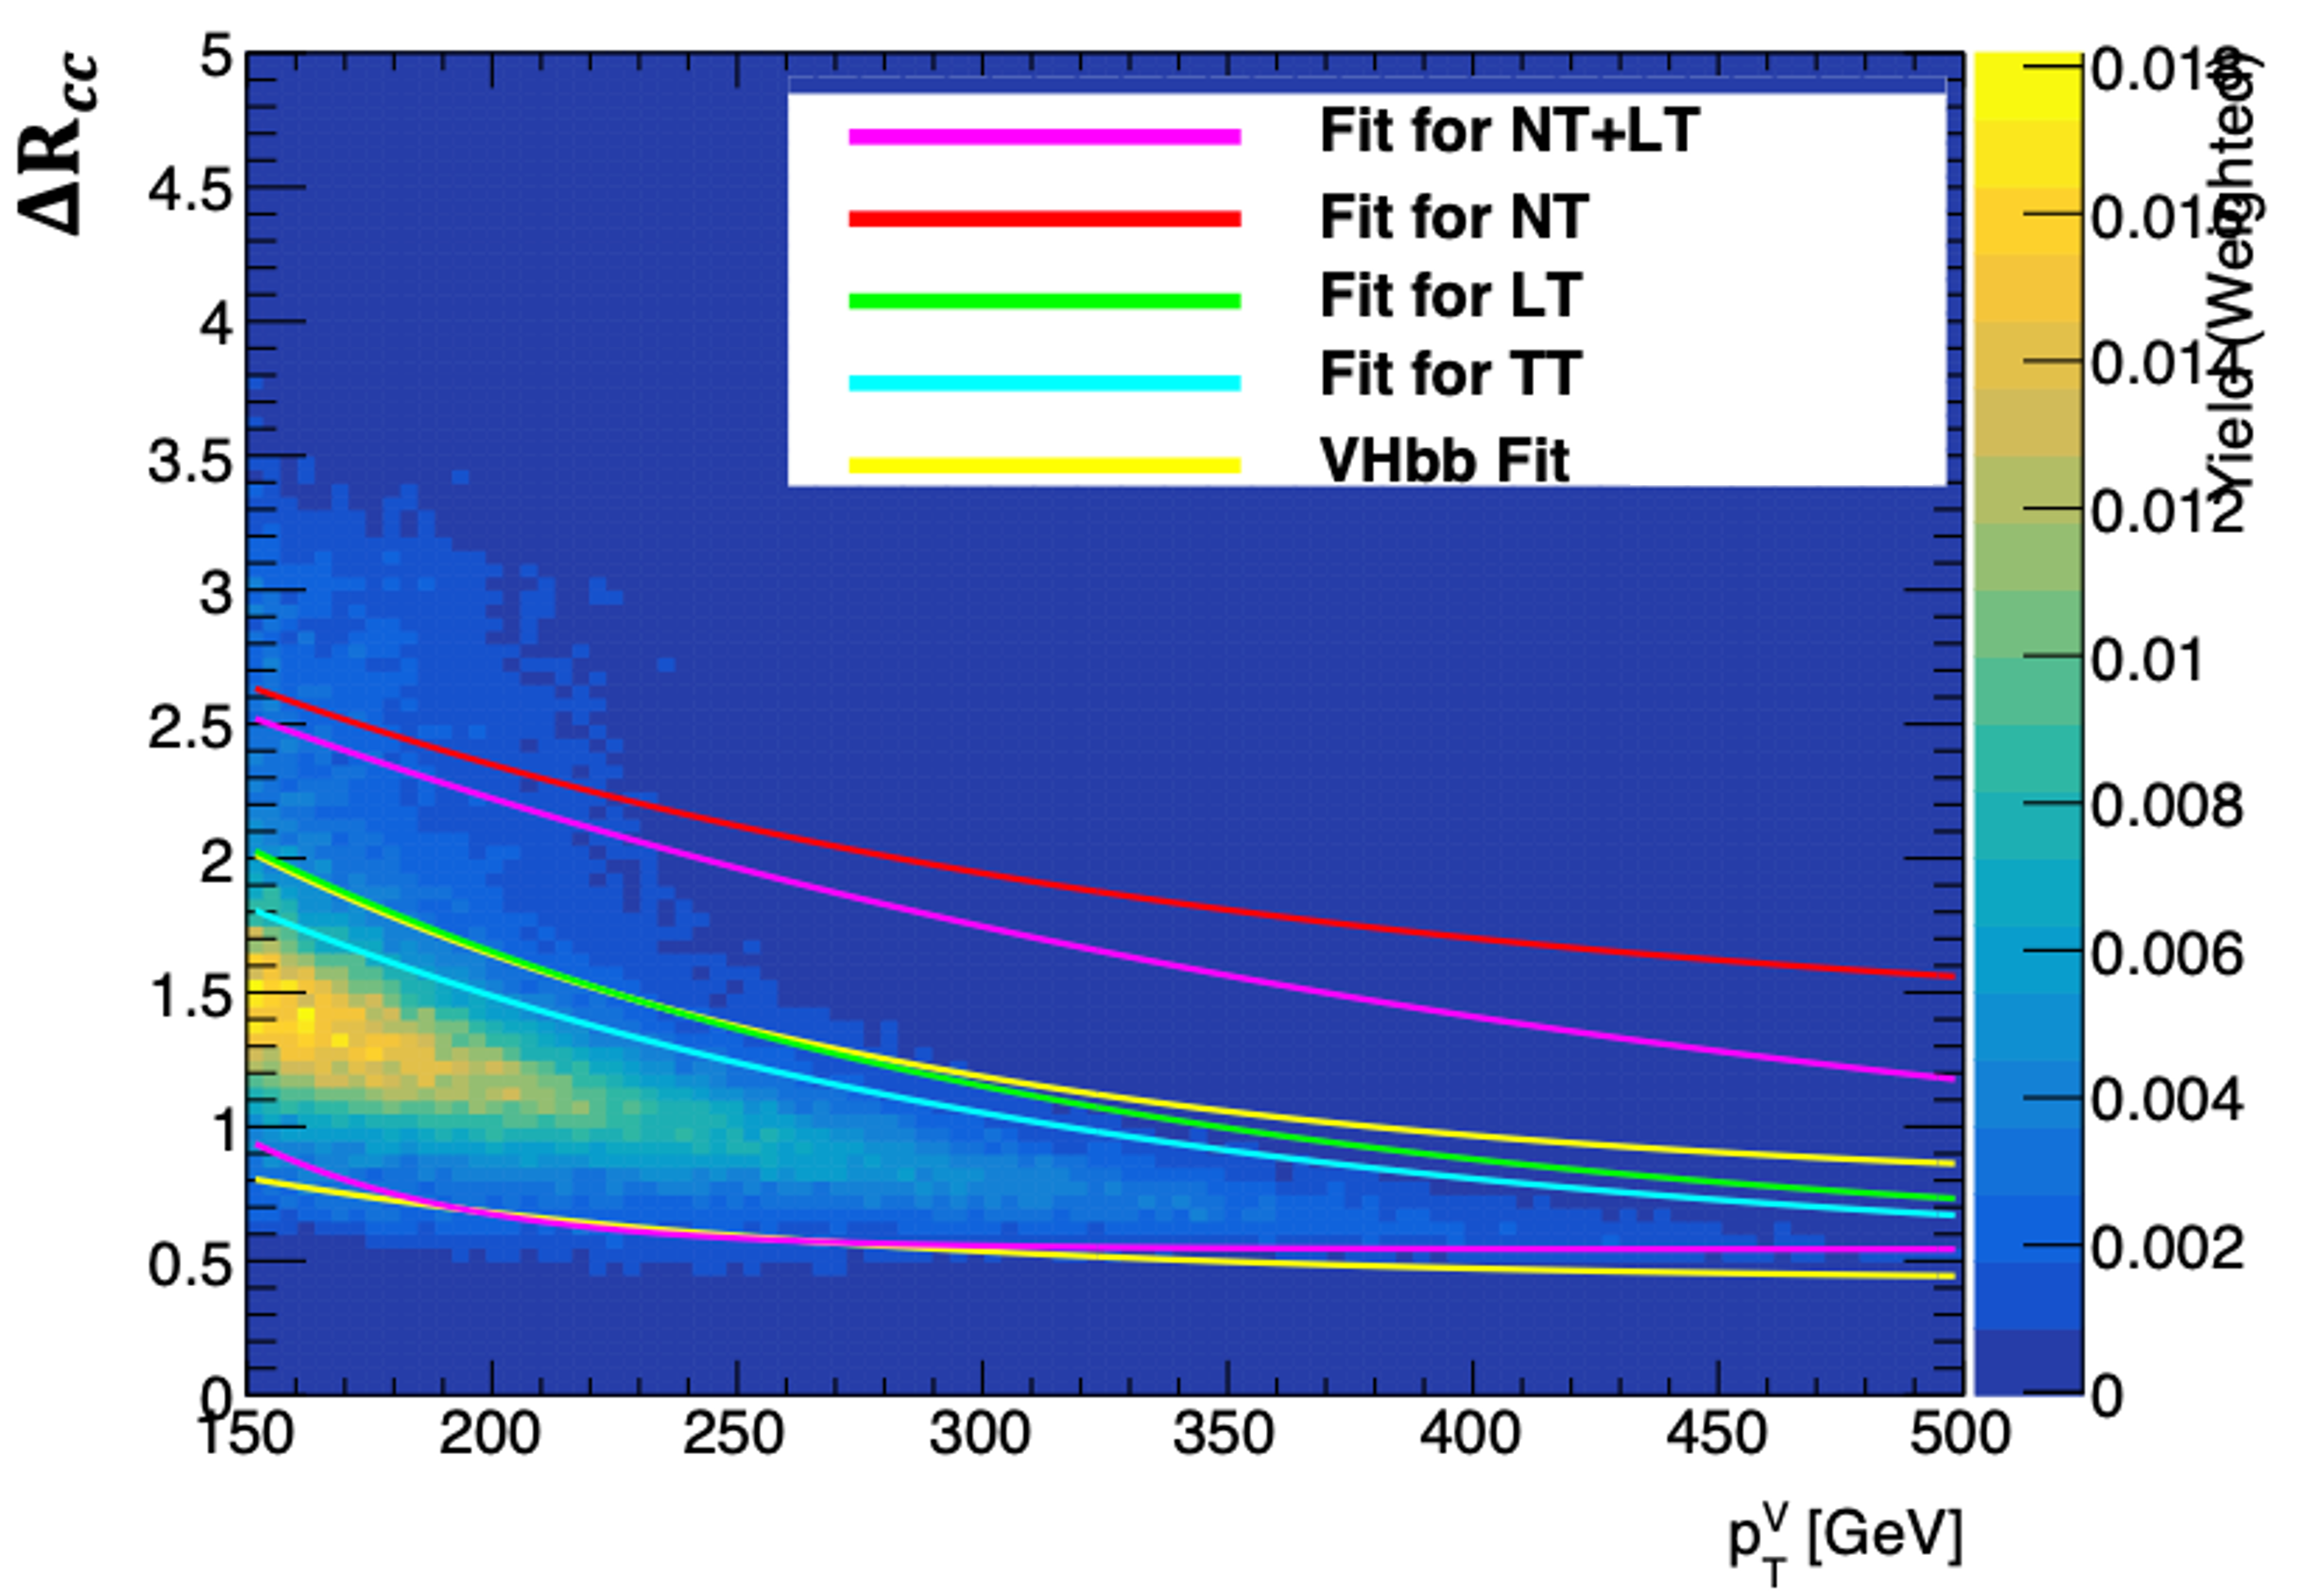
\includegraphics[width=0.48\textwidth]{Images/VH/dRccpTV/sr2.png}
\caption{The $p_T^V$-$\Delta R_{c\bar{c}}$ 2D-histograms showing the signal yield of the 1-lepton $VH(H\rightarrow c\bar{c})$, for the 2-jet (left) and 3-jet (right) signal regions. The lines are the results of fitting the $\Delta R_{c\bar{c}}-p_T^V$ cuts for various signal tags, with the yellow curve showing the $VH(H\rightarrow b\bar{b})$ $p_T^V$-$\Delta R_{b\bar{b}}$ cut.} 
\label{fig:drccptvCutsVHcc}
\end{figure}